\documentclass[a4paper,12pt]{article}
\usepackage[utf8]{inputenc}
\usepackage[spanish]{babel}
\usepackage{graphicx}
\usepackage{geometry}
\usepackage{color}
\usepackage{sectsty}
\usepackage{titlesec}
\usepackage{hyperref}

% Configuración de márgenes
\geometry{left=2cm, right=2cm, top=2cm, bottom=2cm}

% Colores personalizados
\definecolor{darkred}{RGB}{139,0,0}
\definecolor{gold}{RGB}{212,175,55}

% Estilo de secciones
\sectionfont{\color{darkred}\bfseries\Large}
\subsectionfont{\color{gold}\bfseries\large}

% Encabezado y pie de página
\usepackage{fancyhdr}
\pagestyle{fancy}
\fancyhf{}
\fancyhead[L]{
\includegraphics[width=3cm]{logo.png}} % Reemplaza 'logo.png' con el logo de tu organización
\fancyhead[R]{\textbf{Carpeta Artística}}
\fancyfoot[C]{\thepage}

\begin{document}

\begin{center}
    \huge \textbf{Talleres de Baile y Coreografía} \\
    \vspace{0.5cm}
    \large \textit{Explora la riqueza del baile y fandango tradicional de la Tierra Caliente}
\end{center}

\vspace{1cm}

\section*{Introducción}
Bienvenido a nuestros talleres especializados en el baile y fandango tradicional de la Tierra Caliente. Diseñados para todos los niveles, estos talleres te permitirán sumergirte en la cultura y las técnicas que hacen único a este arte.

\section{Taller de Baile y Fandango Tradicional}
\begin{itemize}
    \item \textbf{Descripción:} Aprende los pasos, ritmos y expresiones del fandango tradicional de la Tierra Caliente. Ideal para principiantes y bailarines intermedios.
    \item \textbf{Duración:} 8 semanas
    \item \textbf{Horario:} Martes y Jueves de 18:00 a 20:00
    \item \textbf{Ubicación:} Centro Cultural \emph{La Tierra Caliente}, Calle Principal 123
    \item \textbf{Costo:} \$200 por participante
    \item \textbf{Inscripciones:} \href{mailto:contacto@tierra-caliente.com}{contacto@tierra-caliente.com} | Tel: +123 456 7890
\end{itemize}

\begin{center}
    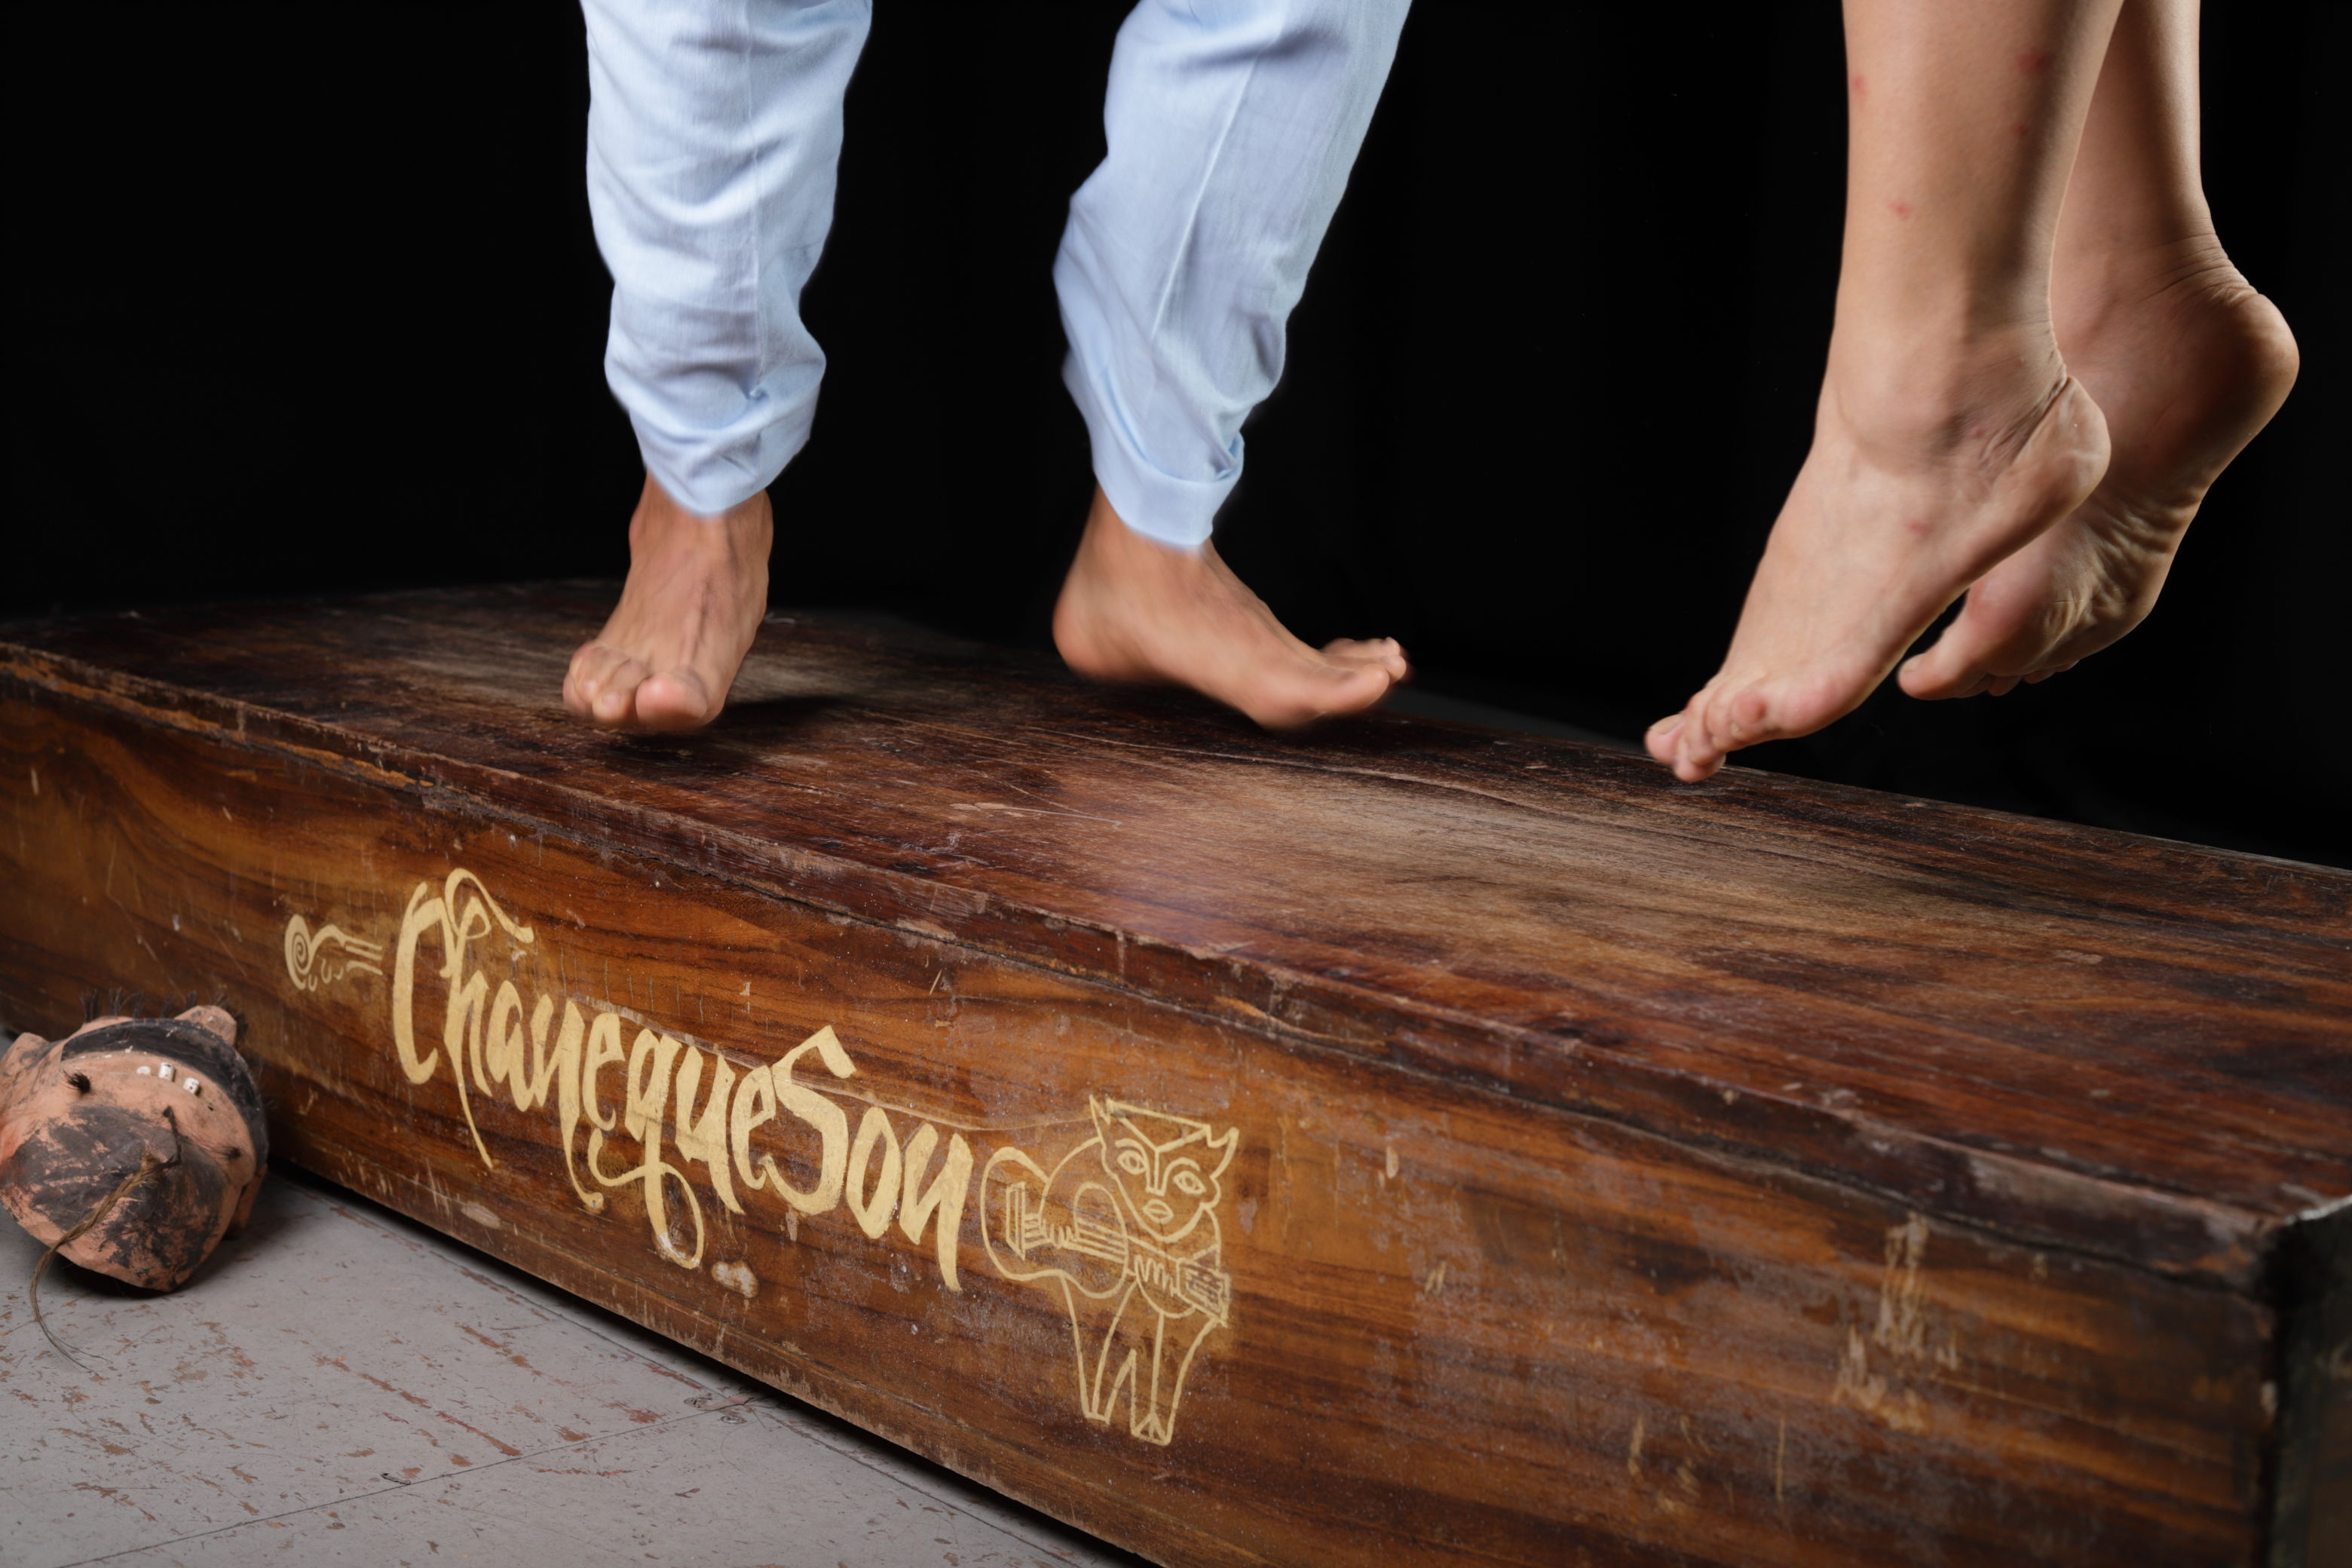
\includegraphics[width=0.8\textwidth]{IMG_4296.jpg} % Reemplaza con una imagen relevante
\end{center}

\section{Taller de Montaje y Diseño de Coreografías}
\begin{itemize}
    \item \textbf{Descripción:} Desarrolla tus habilidades en la creación de coreografías basadas en el baile y fandango tradicional. Aprende a diseñar presentaciones únicas y expresivas.
    \item \textbf{Duración:} 10 semanas
    \item \textbf{Horario:} Sábados de 10:00 a 14:00
    \item \textbf{Ubicación:} Estudio de Danza \emph{Arte Vivo}, Avenida Secundaria 456
    \item \textbf{Costo:} \$300 por participante
    \item \textbf{Inscripciones:} \href{mailto:contacto@tierra-caliente.com}{contacto@tierra-caliente.com} | Tel: +123 456 7890
\end{itemize}

\begin{center}
    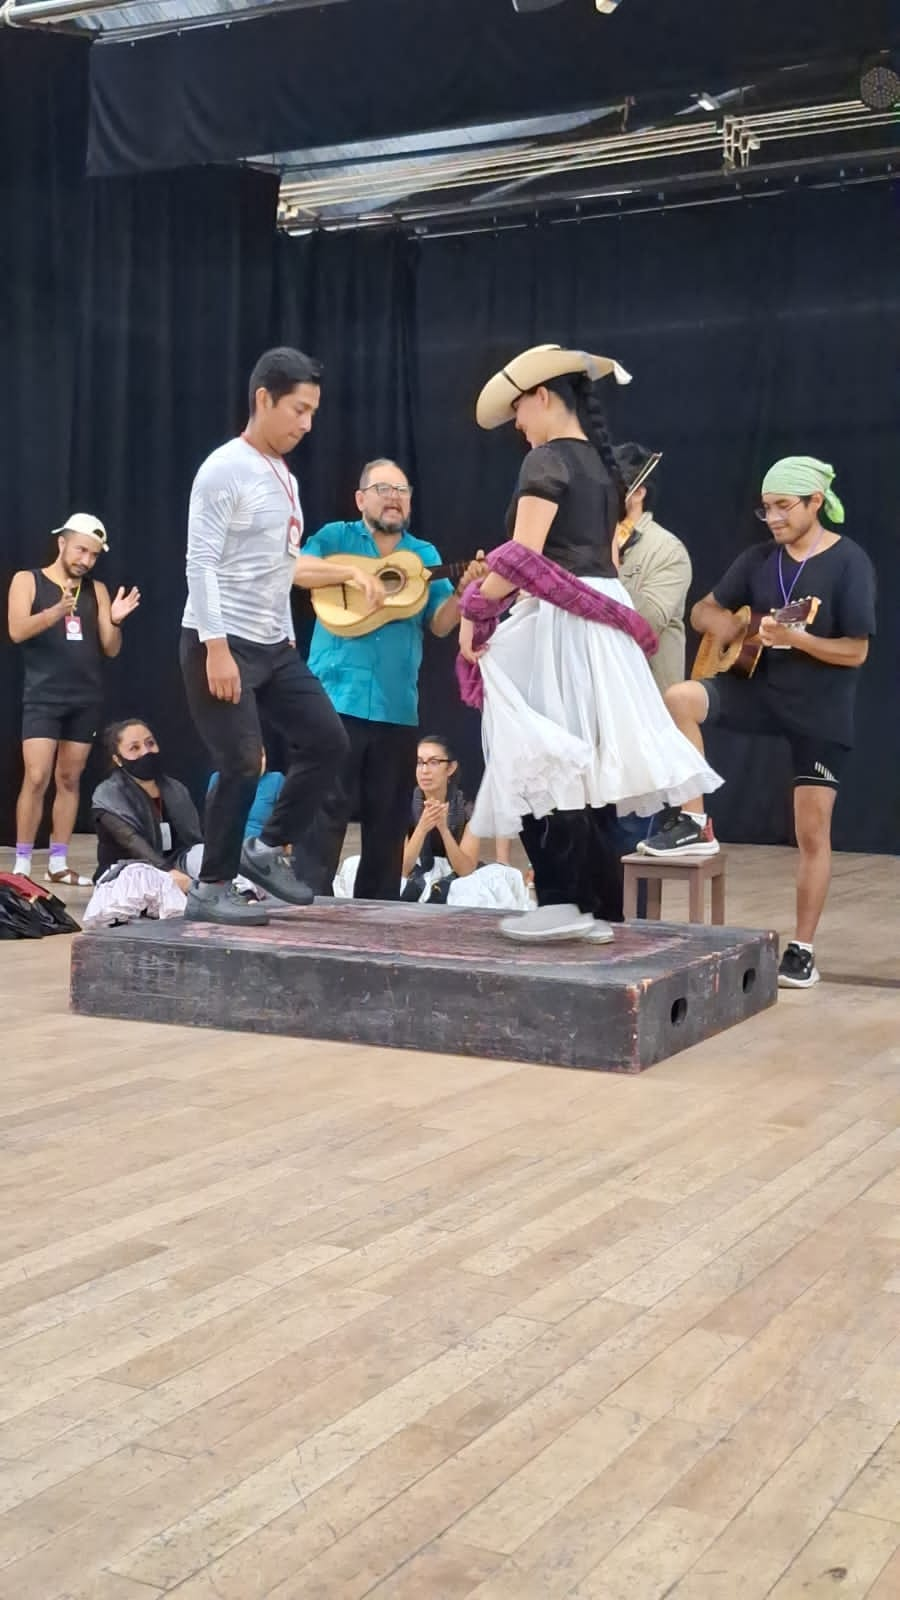
\includegraphics[width=0.8\textwidth]{baile.jpg} % Reemplaza con una imagen relevante
\end{center}

\section*{Beneficios de Participar}
\begin{itemize}
    \item \textbullet{} Inmersión cultural profunda
    \item \textbullet{} Instructores profesionales
    \textbullet{} Materiales y recursos exclusivos
    \item \textbullet{} Certificado de participación
\end{itemize}

\section*{Testimonios}
\textit{"Participar en estos talleres ha enriquecido mi conocimiento y pasión por el fandango. Los instructores son excepcionales y el ambiente es muy acogedor."} \\
-- \textbf{María López}, Participante 2023

\section*{Contacto y Redes Sociales}
- \textbf{Correo Electrónico:} \href{mailto:contacto@tierra-caliente.com}{contacto@tierra-caliente.com} \\
- \textbf{Teléfono:} +123 456 7890 \\
- \textbf{Facebook:} \href{https://facebook.com/tierra-caliente}{facebook.com/tierra-caliente} \\
- \textbf{Instagram:} \href{https://instagram.com/tierra.caliente}{@tierra.caliente}

\end{document}
